\documentclass{article}

% NeurIPS 2024 (final, non-anonymous)
\usepackage[final]{neurips_2024}

% Replace the NeurIPS footer with the course name
\makeatletter
\renewcommand{\@noticestring}{IEOR 6616: Convex Optimization --- Programming Project}
\makeatother

\usepackage[utf8]{inputenc}
\usepackage[T1]{fontenc}
\usepackage{hyperref}
\usepackage{url}
\usepackage{booktabs}
\usepackage{amsfonts}
\usepackage{amsmath}
\usepackage{amssymb}
\usepackage{nicefrac}
\usepackage{microtype}
\usepackage{xcolor}
\usepackage{graphicx}
\usepackage{subcaption}
\usepackage{caption}
\usepackage{natbib}

\title{Computational Optimal Transport: \\
  LP, Quadratic, and Entropic Regularizations}

\author{%
  Jiayi Chen \\
  Columbia UNI: \texttt{JC6601}\\
  \texttt{jc6601@columbia.edu}
}

\begin{document}
\maketitle

\begin{abstract}
We study the discrete optimal transport (OT) problem on random 2D point
clouds and compare three solver paradigms for the linear-programming
formulation (simplex, interior point, primal--dual hybrid gradient),
two algorithms for the quadratically regularized OT (ADMM and IPM), and
the Sinkhorn matrix-scaling algorithm for the entropy-regularized OT.
We verify all regularized variants converge to the LP optimum
$W_{\mathrm{LP}}$ as the regularization vanishes, and we compare the
discrete OT cost with the closed-form Bures--Wasserstein
$W_2^2$ for two 2D Gaussians.  Reproduction instructions are in the
README of the accompanying repository.
\end{abstract}

\section{Setup and notation}
\label{sec:setup}

Let $\{x_i\}_{i=1}^n \!\sim\! \mathcal N(\mu_1,\Sigma_1)$ and
$\{y_j\}_{j=1}^n \!\sim\! \mathcal N(\mu_2,\Sigma_2)$ with
$\mu_1\!=\!(0,0)$, $\mu_2\!=\!(4,3)$,
$\Sigma_1\!=\!\bigl[\!\begin{smallmatrix}1&0.6\\0.6&1.2\end{smallmatrix}\!\bigr]$,
$\Sigma_2\!=\!\bigl[\!\begin{smallmatrix}1.5&-0.7\\-0.7&1\end{smallmatrix}\!\bigr]$.
Both covariances are non-diagonal; uniform weights $a=b=\tfrac1n\mathbf 1$;
quadratic cost $C_{ij}=\|x_i-y_j\|_2^2$.  We fix the random seed for
reproducibility.  The transportation polytope is
$U(a,b)=\{P\!\in\!\mathbb R_{\ge 0}^{n\times n}\!:\!P\mathbf 1\!=\!a,\;
P^{\!\top}\!\mathbf 1\!=\!b\}$.

\section{Part 1: Three LP solver paradigms}
\label{sec:part1}

We solve $W_{\mathrm{LP}} = \min_{P\in U(a,b)}\langle C, P\rangle$ in
standard form (vectorize $P$, sparse marginal matrix in
$\mathbb R^{(2n)\times n^2}$).  Solvers used:
\textbf{Simplex}=\texttt{scipy.optimize.linprog} with HiGHS-DS,
\textbf{IPM}=HiGHS-IPM, \textbf{PDLP}=Google's PDLP via
\texttt{ortools.pdlp.python} (PDHG with adaptive step sizes,
preconditioning and restarts \cite{applegate2021pdlp,chambolle2011first}).
We verify correctness on $n\!\in\!\{3,4\}$: simplex and IPM agree to
machine precision.

\paragraph{Optional: a from-scratch PDHG.}
We implemented the saddle-point PDHG of \S4 of the handout in NumPy
with $\tau\!=\!\sigma\!=\!\tfrac{0.99}{\sqrt{m+n}}$ (so
$\tau\sigma\|K\|^2\!<\!1$ for $K(P)\!=\!(P\mathbf 1, P^{\!\top}\!\mathbf 1)$).
For the Frobenius/$\ell_2$ operator norm, $\|K\|^2\!=\!m+n$, attained
by a constant matrix.  Two modifications were needed: rescale
$C\!\leftarrow\!C/\|C\|_\infty$ so primal/dual scales match, and
restart from the running average every 2000 steps---the lessons of
PDLP \cite{applegate2021pdlp,lu2025overview}.  We then reach
$\|P\mathbf 1\!-\!a\|_1\!+\!\|P^\top\mathbf 1\!-\!b\|_1\!<\!10^{-5}$
in 13\,200 iterations at $n\!=\!200$ (Fig.~\ref{fig:part1pdhg}).

\paragraph{Results.}
Table~\ref{tab:part1} summarizes wall time and accuracy at
$n\!\in\!\{50,100,200,500\}$ on a single CPU; Fig.~\ref{fig:part1timing}
plots time vs.\ $n$ on log--log axes.
On CPU, IPM (HiGHS) is fastest except for an essentially tied $n\!=\!50$
case, and scales roughly as $O(n^{2.5})$ in our range.  Simplex (HiGHS-DS) catches IPM at small $n$
but explodes at $n\!=\!500$ ($25\,$s), reflecting the combinatorial
worst case of pivoting.  PDLP, designed for very large LPs, is
competitive (8\,s at $n\!=\!500$) but not best on CPU---its real
strength is GPU vectorisation of the per-iteration work.  Our custom
NumPy PDHG is uniformly slower because we lack PDLP's adaptive step
sizes and Ruiz preconditioning.  Critically, all three high-accuracy
solvers (Simplex, IPM, PDLP) agree on $W_{\mathrm{LP}}$ to
$10^{-10}$ on small/medium instances; PDLP's first-order terminal
accuracy degrades mildly to a $4\!\cdot\!10^{-8}$ cost gap at
$n\!=\!500$.  Our PDHG agrees to $\sim\!10^{-5}$.

\begin{table}[t]
\centering
\caption{Part 1 -- LP solvers on random Gaussian point clouds (seed $0$).
Marginal violation is $\|P\mathbf 1-a\|_1+\|P^{\!\top}\!\mathbf 1-b\|_1$;
cost gap is $\langle C,P\rangle - W_{\mathrm{LP}}$ where $W_{\mathrm{LP}}$
is the simplex/IPM optimum (which agree to machine precision).  The
reference optima for $n=50,100,200,500$ are $26.99$, $25.48$, $25.06$,
and $24.49$.}
\label{tab:part1}
\scriptsize
\setlength{\tabcolsep}{3pt}
\begin{tabular}{l rrrr rrrr rrrr}
\toprule
& \multicolumn{4}{c}{Wall time (s)}
& \multicolumn{4}{c}{Marginal violation}
& \multicolumn{4}{c}{Cost gap to $W_{\mathrm{LP}}$} \\
\cmidrule(lr){2-5}\cmidrule(lr){6-9}\cmidrule(lr){10-13}
$n$ & 50 & 100 & 200 & 500
    & 50 & 100 & 200 & 500
    & 50 & 100 & 200 & 500 \\
\midrule
Simplex (HiGHS-DS)
  & $0.010$ & $0.080$ & $0.96$ & $25.03$
  & $\!10^{-16}\!$ & $\!10^{-16}\!$ & $\!10^{-16}\!$ & $\!10^{-16}\!$
  & $0$ & $0$ & $0$ & $0$ \\
IPM (HiGHS-IPM)
  & $0.011$ & $0.054$ & $0.25$ & $2.44$
  & $\!10^{-16}\!$ & $\!10^{-16}\!$ & $\!10^{-16}\!$ & $\!10^{-16}\!$
  & $0$ & $0$ & $0$ & $0$ \\
PDLP (OR-Tools)
  & $0.022$ & $0.151$ & $0.68$ & $8.02$
  & $\!3\!\cdot\!10^{-14}\!$ & $\!6\!\cdot\!10^{-14}\!$ & $\!5\!\cdot\!10^{-11}\!$ & $\!6\!\cdot\!10^{-13}\!$
  & $\!10^{-13}\!$ & $\!10^{-13}\!$ & $\!8\!\cdot\!10^{-10}\!$ & $\!4\!\cdot\!10^{-8}\!$ \\
PDHG (custom NumPy)
  & $0.092$ & $0.357$ & $1.52$ & $33.72$
  & $\!4\!\cdot\!10^{-6}\!$ & $\!10^{-5}\!$ & $\!10^{-5}\!$ & $\!10^{-4}\!$
  & $\!2\!\cdot\!10^{-4}\!$ & $\!10^{-4}\!$ & $\!10^{-4}\!$ & $\!3\!\cdot\!10^{-4}\!$ \\
\bottomrule
\end{tabular}
\end{table}

\section{Part 2: Quadratic regularization}
\label{sec:part2}

We solve $\min_{P\in U(a,b)}\langle C,P\rangle + \tfrac\lambda 2\|P\|_F^2$.
\textbf{ADMM via OSQP} (CVXPY) and \textbf{IPM via Clarabel} (CVXPY)
gave costs $25.067388$ and $25.064712$ respectively at $\lambda\!=\!0.1$,
$n\!=\!200$, with wall times $6.07$\,s (OSQP) vs.\ $0.31$\,s (Clarabel).
The IPM is twenty times faster on this problem because the QP is small,
strictly convex, and well-conditioned: Newton steps converge in $\sim\!15$
iterations.  ADMM via OSQP requires many more iterations and pays for
the upfront KKT factorization.

\paragraph{Custom ADMM and the role of $\rho$.}
We also implemented the splitting from the handout in NumPy with one
modification that drastically improved convergence: we put the
nonnegativity constraint in the $P$-block (so the $P$-update has the
closed-form clip given in eq.~(4) of the handout) and put the
\emph{affine} marginal constraint in the $Q$-block (so the $Q$-update
becomes the closed-form orthogonal projection onto
$\{Q\!:\!Q\mathbf 1\!=\!a,\,Q^{\!\top}\!\mathbf 1\!=\!b\}$, no Dykstra
inner loop required).  Both blocks then have $O(n^2)$ closed-form updates.
Fig.~\ref{fig:part2rho} shows the achieved marginal violation after
$20\,000$ iterations as a function of $\rho$ at $\lambda\!=\!0.1$,
$n\!=\!200$: convergence requires $\rho \gtrsim n$ (e.g.\ $\rho\!=\!300$
suffices), because $a$ and $b$ scale as $1/n$ while $C$ has $O(1)$
entries, so the dual updates need to be amplified to balance.
This matches the well-known sensitivity of vanilla ADMM to the
penalty $\rho$ and motivates the adaptive schemes used by OSQP.

\paragraph{Regularization path.}
Fig.~\ref{fig:part2path} plots the gap $\langle C,P^*_\lambda\rangle\!-\!W_{\mathrm{LP}}$
on log--log axes for $\lambda\!\in\![10^{-3},10]$.  The gap shrinks
monotonically and is tiny ($<\!10^{-2}$) over the full range; this is
because $\|P^*\|_F^2 \approx 1/n$ for the sparse LP solution, so
$\tfrac\lambda 2\|P\|_F^2$ is at most $\sim 0.025$ even at $\lambda\!=\!10$.
Unlike entropic regularization, the quadratic penalty still admits
exact zeros: the KKT condition reduces to the soft-thresholding
$P^*_{ij}\!=\!\max\bigl(0, (f_i+g_j-C_{ij})/\lambda\bigr)$, so entries
with $f_i+g_j<C_{ij}$ are pinned to zero (Fig.~\ref{fig:couplings},
center-left).

\section{Part 3: Entropic regularization (Sinkhorn)}
\label{sec:part3}

We solve $\min_{P\in U(a,b)}\langle C,P\rangle + \lambda\sum_{ij}P_{ij}\log P_{ij}$
with three implementations: (i) the POT library
(\texttt{ot.sinkhorn}, log-domain), (ii) our own log-domain Sinkhorn in
NumPy, and (iii) a generic conic solver through CVXPY using
\texttt{cp.entr} (the exponential cone)
\cite{cuturi2013sinkhorn,peyre2019computational}.  The two candidate
conic backends play different algorithmic roles: Clarabel is a true
interior-point conic solver (analogous to HiGHS-IPM in Part~1, but for
the exponential cone), while SCS is a first-order operator-splitting
conic solver, closer in spirit to ADMM than to an IPM.
We work in the log domain throughout: at $\lambda\!=\!0.01$ the entries
$\exp(-C/\lambda)$ underflow at double precision, so naive
matrix-form Sinkhorn fails.  At $n\!=\!200$ our custom Sinkhorn
matches POT to $10^{-5}$ in cost; convergence is fast at $\lambda\!=\!1$
(33 iterations to reach $10^{-6}$ marginal violation) and slows as
$\lambda$ decreases (318 iterations at $\lambda\!=\!0.1$; at
$\lambda\!=\!0.01$, $20\,000$ iterations still leave a residual of
$1.7\!\cdot\!10^{-6}$, Fig.~\ref{fig:part3conv}).

\paragraph{Sinkhorn vs.\ conic IPM (Clarabel) and FO conic (SCS), $\lambda\!=\!0.1$.}
Table~\ref{tab:part3} summarizes the three solvers across $n$ on the
same seed-0 instances.  Wall times are medians of three timed repeats
after one warm-up solve, and include library/Python overhead.  The
small cases show that conic solvers can be competitive: Clarabel is
fastest at $n\!=\!30$ and $n\!=\!100$.  Sinkhorn's time is not monotone
in $n$ because the number of scaling iterations is strongly
instance-dependent; the $n\!=\!100$ instance is harder than the
$n\!=\!200$ instance at this $\lambda$ (22\,283 iterations vs.\ 318).
At $n\!=\!200$, however,
Clarabel fails on the $40\,000$-entry exponential cone and SCS is
roughly $60\times$ slower than Sinkhorn while giving the same transport
cost to about $5\!\cdot\!10^{-3}$.

\begin{table}[h]
\centering
\caption{Part 3 -- entropic OT at $\lambda\!=\!0.1$: custom log-domain
Sinkhorn vs.\ Clarabel (interior-point conic) vs.\ SCS (first-order
operator-splitting conic).  Timings are median wall times over three
post-warm-up repeats on the same seed-0 instance; the middle block
shows Sinkhorn scaling iterations to reach $10^{-6}$ marginal violation.}
\label{tab:part3}
\scriptsize
\setlength{\tabcolsep}{2pt}
\begin{tabular}{l rrrr rrrr rrrr}
\toprule
& \multicolumn{4}{c}{Wall time (s)}
& \multicolumn{4}{c}{Sinkhorn iterations}
& \multicolumn{4}{c}{Cost $\langle C,P^*\rangle$} \\
\cmidrule(lr){2-5}\cmidrule(lr){6-9}\cmidrule(lr){10-13}
$n$           & 30 & 50 & 100 & 200 & 30 & 50 & 100 & 200 & 30 & 50 & 100 & 200 \\
\midrule
Sinkhorn (custom log)
  & $0.259$ & $0.028$ & $3.20$ & $0.161$
  & $8931$ & $586$ & $22283$ & $318$
  & $24.831$ & $27.037$ & $25.534$ & $25.132$ \\
Clarabel (IPM conic)
  & $0.021$ & $0.059$ & $0.30$ & FAIL
  & --- & --- & --- & ---
  & $24.831$ & $27.037$ & $25.534$ & --- \\
SCS (FO conic)
  & $0.120$ & $0.258$ & $1.54$ & $10.27$
  & --- & --- & --- & ---
  & $24.832$ & $27.044$ & $25.543$ & $25.138$ \\
\bottomrule
\end{tabular}
\end{table}

\paragraph{Regularization path.}
Fig.~\ref{fig:part3path} shows the cost gap to $W_{\mathrm{LP}}$ on
log--log axes for $\lambda\!\in\![10^{-2},10]$.  The gap closes smoothly
to $\sim\!10^{-3}$ as $\lambda\!\to\!0$.  Note that every Sinkhorn plan
is \emph{mathematically dense}: $P^*_{ij}\!=\!u_iK_{ij}v_j\!>\!0$ for
all $(i,j)$ since $u, v$ are strictly positive at convergence.
The edge counts annotated under Fig.~\ref{fig:couplings} are therefore
only the number of entries above the visualization threshold
$10^{-3}P_{\max}$, not the support of $P^*$.  By contrast the LP plan
is a vertex of $U(a,b)$ and so has at most $2n\!-\!1$ structurally
nonzero entries, and the quadratic plan inherits exact zeros from the
clip $\max(0,\cdot)$ in the soft-thresholding KKT step; both are
genuinely sparse.  Thus at $\lambda\!=\!1$ the Sinkhorn plan has
$\sim\!25\,500$ entries above threshold (effectively dense for plotting),
whereas at $\lambda\!=\!0.01$ only $\sim\!1\,100$ entries remain above
threshold and the plan visually approximates the LP support.

\section{Part 4: Gaussian OT and Bures--Wasserstein}
\label{sec:part4}

For the chosen $\mu_i,\Sigma_i$ the Bures--Wasserstein closed form
$W_2^2 = \|\mu_1-\mu_2\|^2 + \mathrm{tr}\bigl(\Sigma_1+\Sigma_2 -
2(\Sigma_1^{1/2}\Sigma_2\Sigma_1^{1/2})^{1/2}\bigr)$ evaluates to
$25.852$.  We sample $n\!\in\!\{50,100,200,500\}$ points from each
Gaussian and solve the discrete OT LP for $10$ random seeds per $n$
(Fig.~\ref{fig:part4conv}).  Across our finite-sample range
$n\!\le\!500$, the empirical discrete OT cost fluctuates around
$25.32$--$25.40$, i.e.\ slightly below the population value $25.852$.
We interpret this as finite-sample noise rather than a guaranteed
downward bias: the sign and magnitude of the bias in plug-in
empirical OT depend on the distributions and the regime, and in general
one cannot assert that $\mathbb E\,\langle C, P_n^*\rangle$ lies below
$W_2^2$ for all $n$ (a familiar counterexample is two equal
distributions, where $W_2^2\!=\!0$ but $\mathbb E\,\langle C, P_n^*\rangle\!>\!0$).
Asymptotically the plug-in estimator does converge to $W_2^2$
\cite{peyre2019computational}; the trend toward the dashed line in
Fig.~\ref{fig:part4conv} is not visually conclusive at our sample sizes,
though the standard deviation does shrink with $n$ ($1.85\!\to\!0.59$).
Showing convergence cleanly would require substantially larger $n$ and
more seeds.  Fig.~\ref{fig:part4arrows} overlays the LP coupling at
$n\!=\!200$ on the $2$-$\sigma$ Gaussian contour ellipses.

\paragraph{LLM usage and reproduction.}
A coding LLM was used as a pair-programmer for boilerplate (plot
styling, sparse-matrix assembly, \LaTeX\ scaffolding) and surfaced a
bug in the first ADMM splitting; all algorithmic decisions, parameter
sweeps, and analysis are the author's, and every reported number comes
from running the repository.  Reproduction:
\texttt{pip install -r requirements.txt \&\& python run\_all.py}.

\clearpage
{\scriptsize
\setlength{\bibsep}{0pt}
\bibliographystyle{plain}
\bibliography{refs}
}

%%%%%%%%%%%%%%%%%%%%%%%%%%%%%%%%%%%%%%%%%%%%%%%%%%%%%%%
\clearpage
\appendix
\section*{Appendix: Figures}
%%%%%%%%%%%%%%%%%%%%%%%%%%%%%%%%%%%%%%%%%%%%%%%%%%%%%%%

\begin{figure}[h]
\centering
\begin{minipage}[t]{0.49\linewidth}
  \centering
  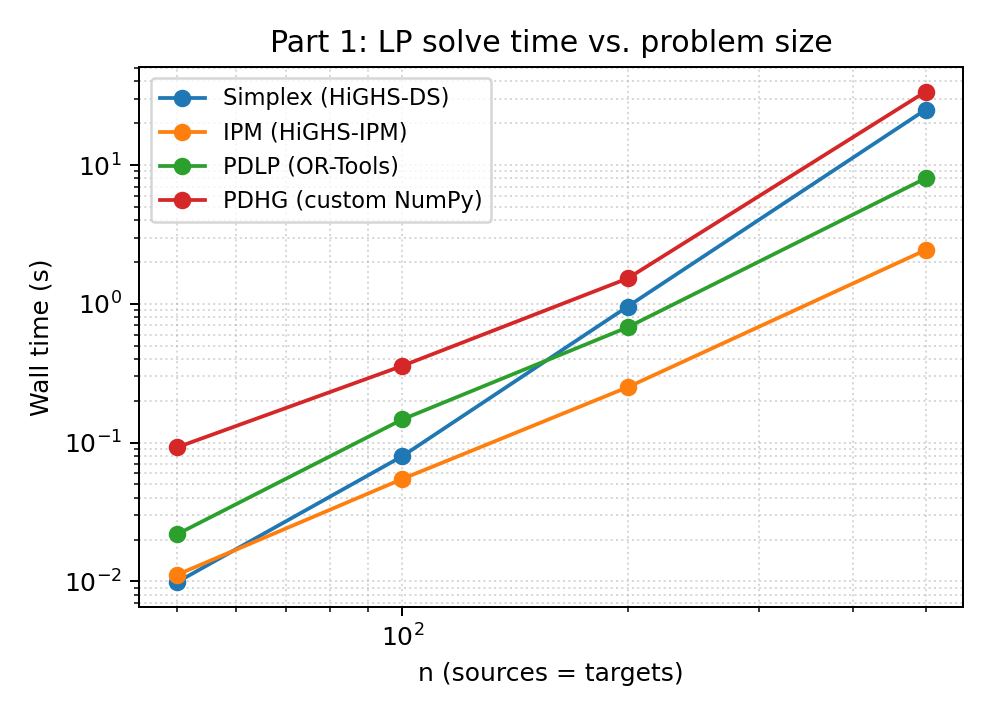
\includegraphics[width=\linewidth]{../results/part1_timing.png}
  \captionof{figure}{Part 1: log--log wall time vs.\ problem size for the
    OT LP. IPM (HiGHS) wins on CPU; simplex blows up at $n\!=\!500$;
    PDLP and our custom NumPy PDHG sit between the two.}
  \label{fig:part1timing}
\end{minipage}\hfill
\begin{minipage}[t]{0.49\linewidth}
  \centering
  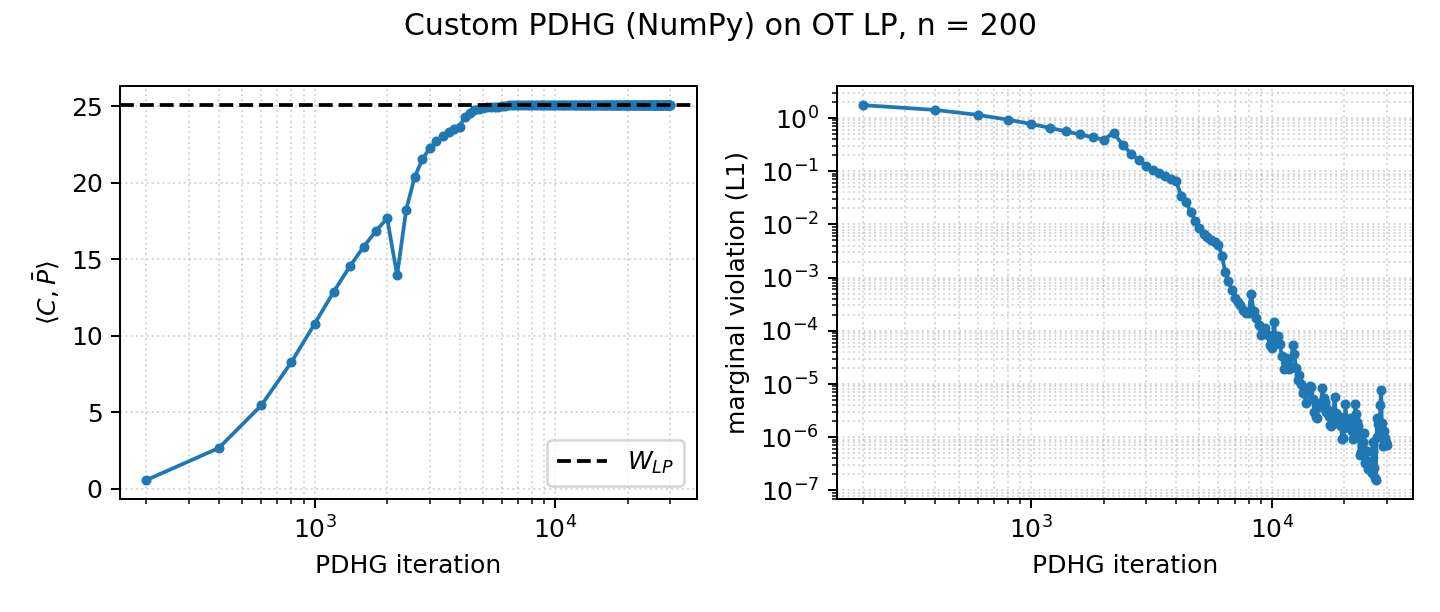
\includegraphics[width=\linewidth]{../results/part1_pdhg_history.png}
  \captionof{figure}{Custom PDHG on the OT LP at $n\!=\!200$: the
    averaged iterate $\bar P$ converges to $W_{\mathrm{LP}}\!=\!25.06$
    (left); the marginal violation reaches $10^{-6}$ in ${\sim}13\,000$
    iterations (right).}
  \label{fig:part1pdhg}
\end{minipage}
\end{figure}

\begin{figure}[h]
\centering
\begin{minipage}[t]{0.49\linewidth}
  \centering
  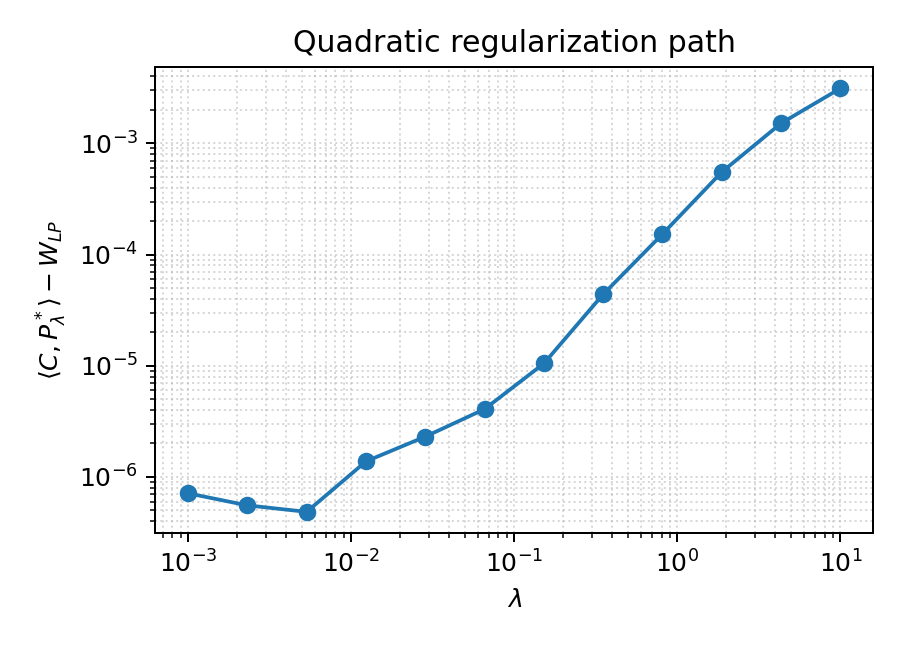
\includegraphics[width=\linewidth]{../results/part2_reg_path.png}
  \captionof{figure}{Quadratic regularization path: cost gap to
    $W_{\mathrm{LP}}$ on log--log axes.  The gap is small over the
    entire range $\lambda\!\in\![10^{-3},10]$ because
    $\|P^*\|_F^2\!\approx\!1/n$ at the LP optimum.}
  \label{fig:part2path}
\end{minipage}\hfill
\begin{minipage}[t]{0.49\linewidth}
  \centering
  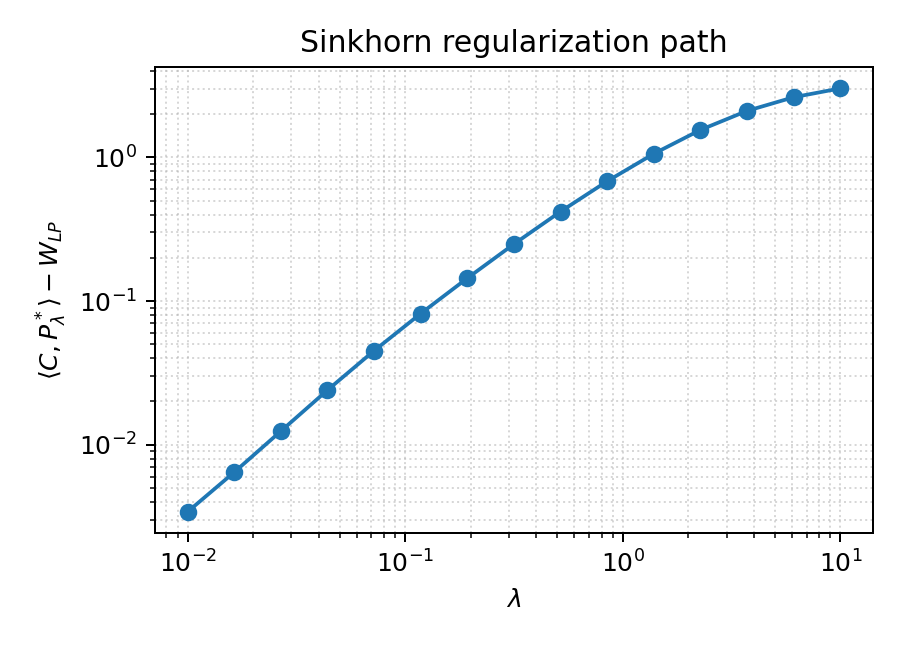
\includegraphics[width=\linewidth]{../results/part3_reg_path.png}
  \captionof{figure}{Sinkhorn regularization path: cost gap to
    $W_{\mathrm{LP}}$ on log--log axes.  Smooth $O(\lambda)$ behaviour
    visible across two decades.}
  \label{fig:part3path}
\end{minipage}
\end{figure}

\begin{figure}[h]
\centering
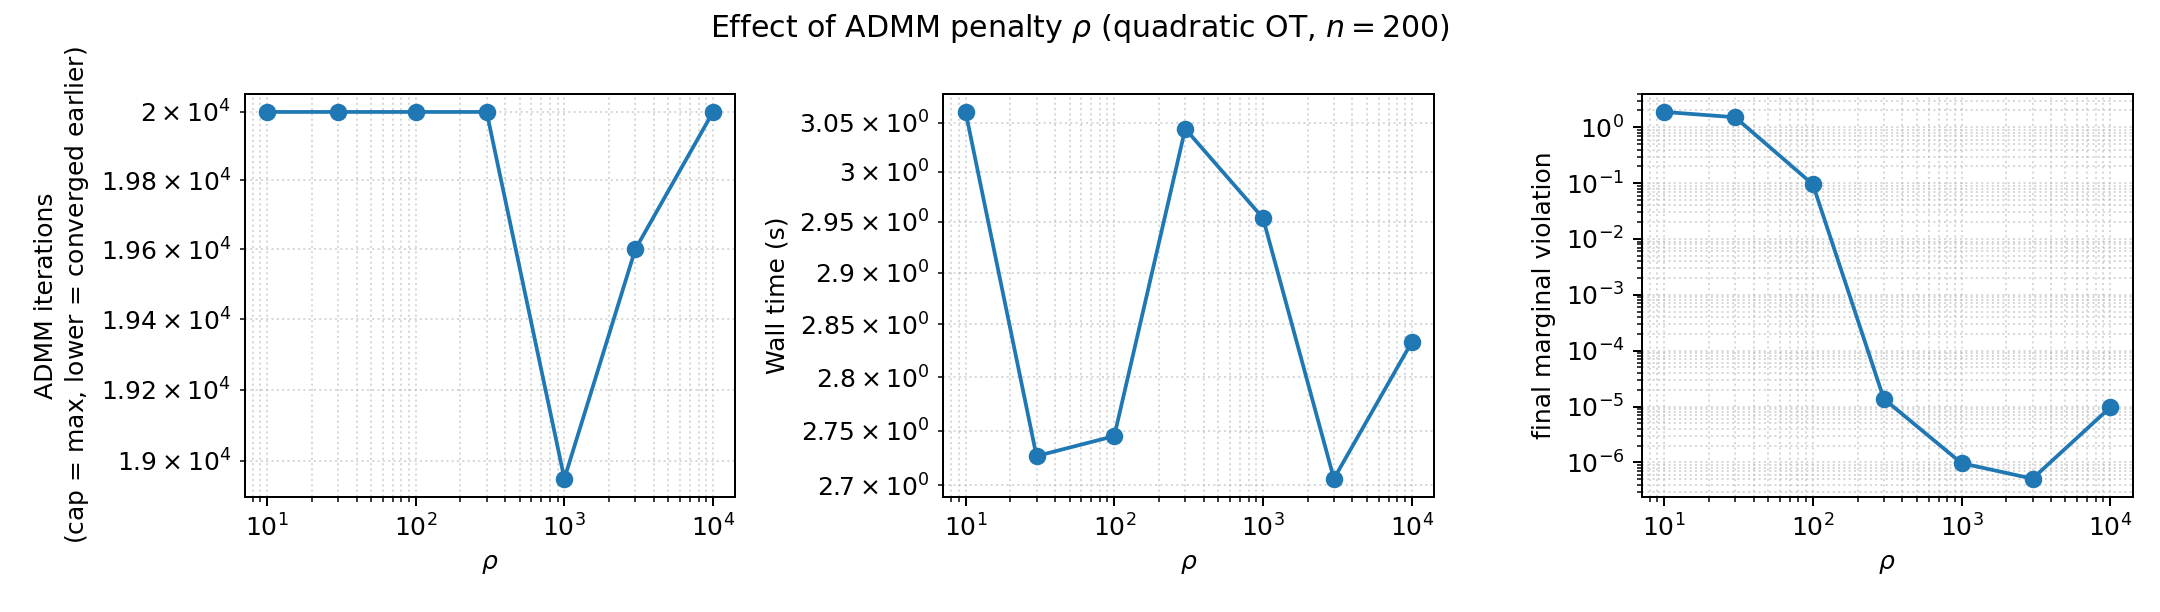
\includegraphics[width=0.95\linewidth]{../results/part2_admm_rho.png}
\caption{Effect of the ADMM penalty $\rho$ in our custom NumPy ADMM
  (quadratic OT, $\lambda\!=\!0.1$, $n\!=\!200$).  Convergence requires
  $\rho \gtrsim n$ (here $\rho\!\ge\!300$); below that, $20\,000$ iterations
  are insufficient and the marginal violation stalls.}
\label{fig:part2rho}
\end{figure}

\begin{figure}[h]
\centering
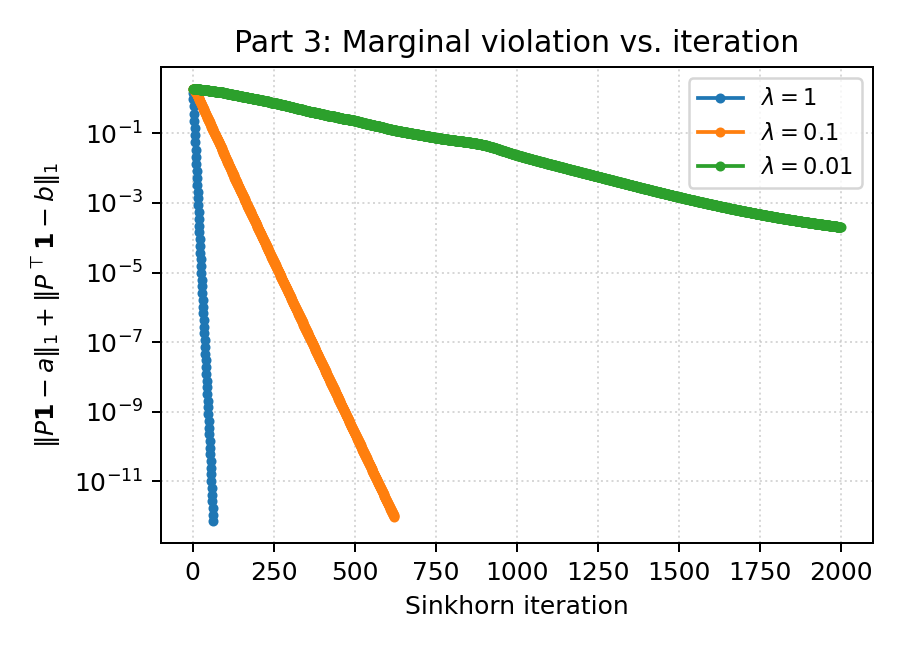
\includegraphics[width=0.6\linewidth]{../results/part3_convergence.png}
\caption{Sinkhorn convergence at $n\!=\!200$ for $\lambda\!\in\!\{1,0.1,0.01\}$.
  Linear convergence in iterates; rate degrades as $\lambda\!\to\!0$.}
\label{fig:part3conv}
\end{figure}

\begin{figure}[h]
\centering
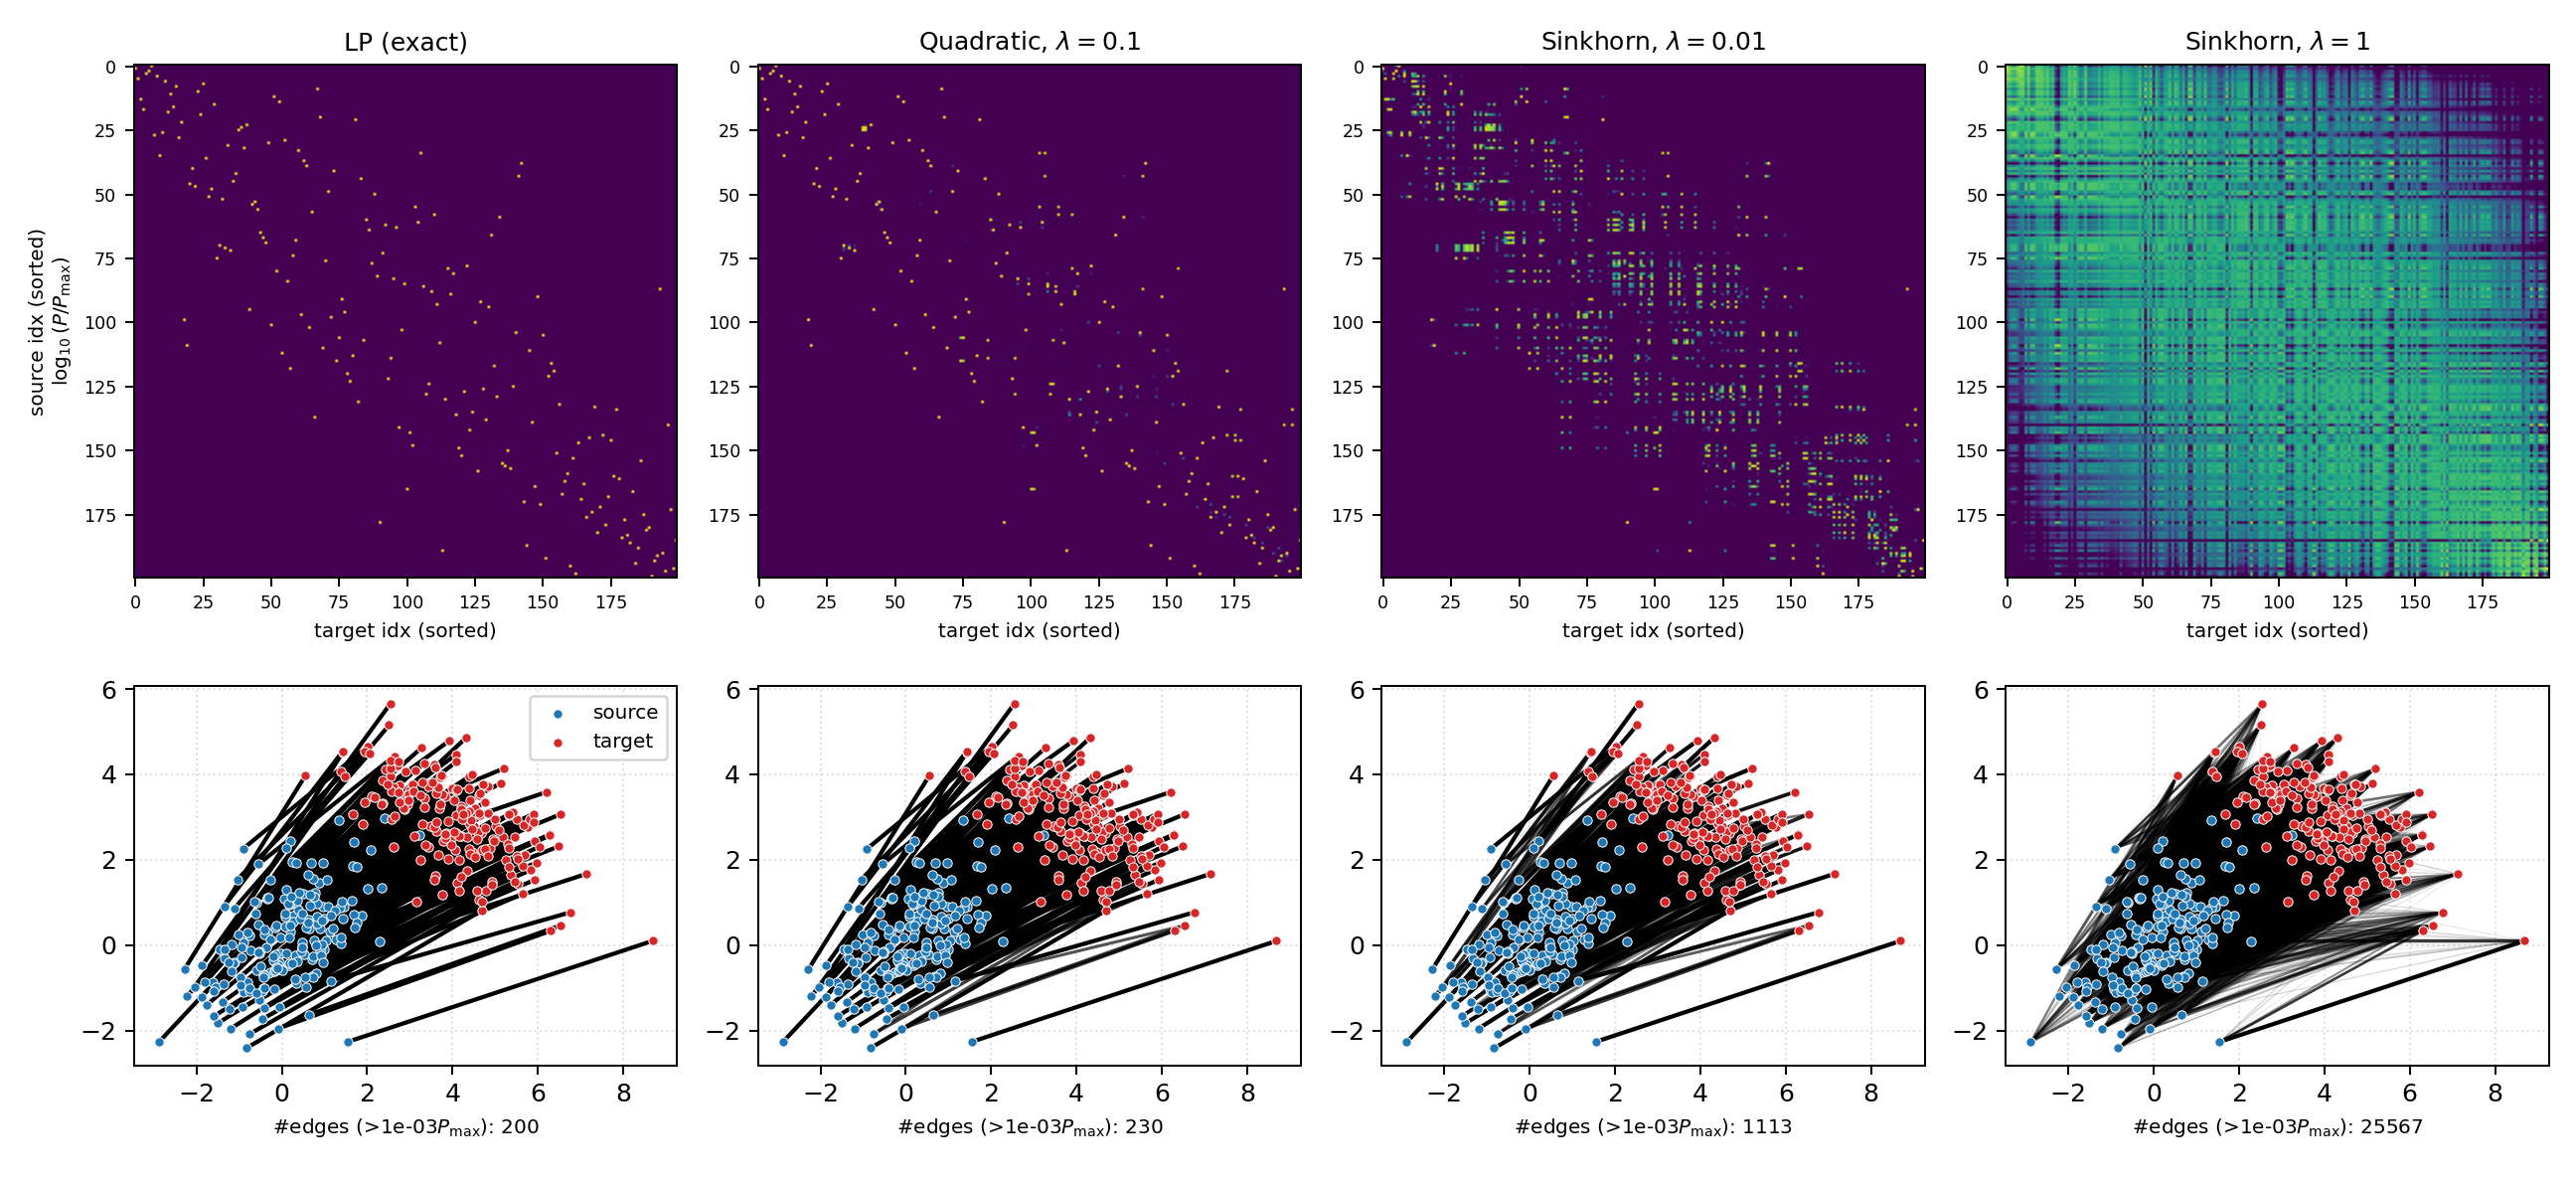
\includegraphics[width=\linewidth]{../results/couplings.png}
\caption{Same point cloud ($n\!=\!200$, seed 0) under four solvers.
  Top row: log-magnitude heatmap of the coupling $P/P_{\max}$ with
  source/target indices sorted by $x$-coordinate.  Bottom row:
  source--target connections weighted by $P_{ij}$.  The number of
  entries \emph{above the visualization threshold} $10^{-3}P_{\max}$
  is annotated below each panel.  The LP and quadratic
  ($\lambda\!=\!0.1$) plans are genuinely sparse (LP at a vertex of
  $U(a,b)$; quadratic gets exact zeros from the soft-thresholding KKT
  step).  Both Sinkhorn plans are mathematically dense
  ($P^*_{ij}\!>\!0$ everywhere); the apparent sparsity at
  $\lambda\!=\!0.01$ ($\approx\!1\,100$ entries above threshold) is
  numerical, not structural.}
\label{fig:couplings}
\end{figure}

\begin{figure}[h]
\centering
\begin{minipage}[t]{0.49\linewidth}
  \centering
  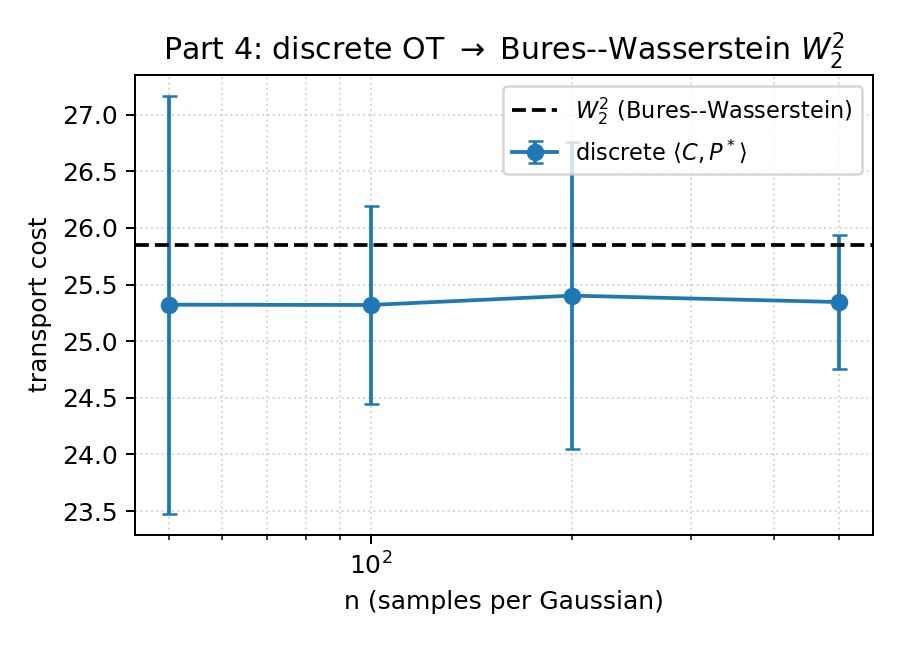
\includegraphics[width=\linewidth]{../results/part4_convergence.png}
  \captionof{figure}{Part 4: discrete OT cost vs.\ $n$, mean $\pm$ one
    standard deviation across $10$ seeds.  Dashed line is the
    Bures--Wasserstein closed form $W_2^2\!=\!25.85$.  In this
    finite-sample range the empirical estimates fluctuate slightly
    below the population value; this should be interpreted as
    finite-sample noise rather than a universal downward bias.
    Standard deviation shrinks with $n$.}
  \label{fig:part4conv}
\end{minipage}\hfill
\begin{minipage}[t]{0.49\linewidth}
  \centering
  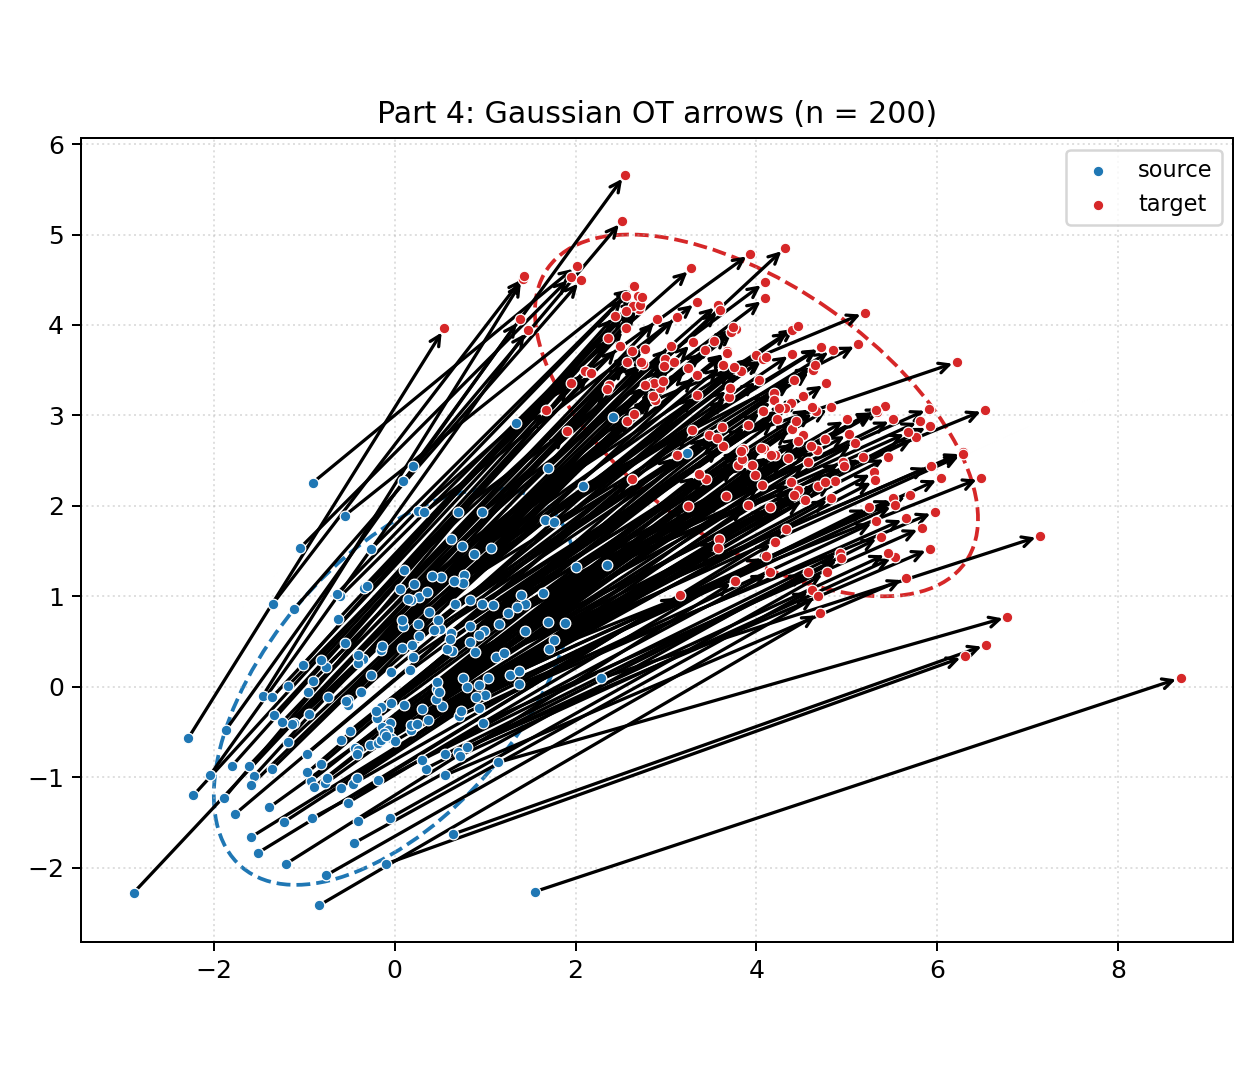
\includegraphics[width=\linewidth]{../results/part4_arrows.png}
  \captionof{figure}{Part 4: LP coupling at $n\!=\!200$ between samples
    of two 2D Gaussians, overlaid on the $2\sigma$ contour ellipses
    (blue source, red target).  Arrow opacity/width is proportional
    to $P_{ij}$.}
  \label{fig:part4arrows}
\end{minipage}
\end{figure}

\end{document}
